\documentclass{beamer}
\usepackage[utf8]{inputenc}
\usepackage{graphicx}
\usetheme{Madrid}

\title{Markdown}
\author{Goran Diklić, Leo Domitrović, Filip Nikolaus}
\date{7.1.2018}

\begin{document}

\maketitle

\newpage

\begin{frame}
\frametitle{Markdown}

\begin{itemize}
\item opisni markup jezik za označavanje teksta
\item jednostavan i čitak
\item Povijest:
\begin{enumerate}
\item 2004. - A. Swartz i J. Gruber kreirali sintaksu jezika Markdown
\item 2012. - standardizacija Markdown jezika - CommonMark
\item 2014. - prva inačica CommonMark-a
\item 2017. - GitHub izdaje specifikaciju za GitHub Flavored Markdown
(GFM) - baza CommonMark
\end{enumerate}

	
\end{itemize}
\end{frame}

\newpage

\begin{frame}
\frametitle{Oblikovanje teksta}
\begin{itemize}
\item podebljavanje i ukošavanje teksta
\item \emph{znakovi: * i  \rule{0.2cm}{0.5pt}}
\item korištenje jednog znakav(* ili \rule{0.2cm}{0.5pt}) - ukošavanje
\item korištenje dva znaka (** ili \rule{0.2cm}{0.5pt} \rule{0.2cm}{0.5pt}) - podebljavanje
\item kombiniranje znakova za oblikovanje riječi i rečenica
\item moguće oblikovati samo jednu riječ, nekoliko riječi ili kompletnu rečenicu
\end{itemize}
\end{frame}

\newpage

\begin{frame}
\frametitle{Podebljavanje teksta - primjeri}

\begin{figure}
\caption{Markdown kod}
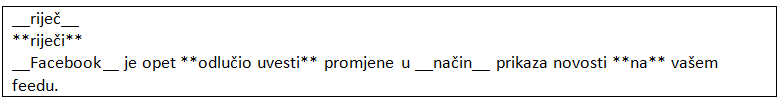
\includegraphics[width = 1.0\linewidth]{/Users/Goran/Documents/GitHub/Markdown/Podebljavanje.png}
\end{figure}

\begin{figure}
\caption{Prikaz}
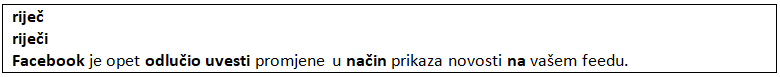
\includegraphics[width = 1.0\linewidth]{/Users/Goran/Documents/GitHub/Markdown/Prikaz1.png}
\end{figure}

\end{frame}







\end{document}